\normalfont\documentclass[letterpaper,11pt]{article}
\usepackage{amsmath, amsfonts,amssymb,latexsym}
\usepackage{fullpage}
\usepackage{parskip}
\usepackage{flexisym}
\usepackage{indentfirst}
\usepackage{graphicx}
\usepackage{algorithm2e}
% \usepackage{algorithm}
\usepackage{algorithmicx}
% \usepackage{algpseudocode}
\usepackage{amsmath}
\begin{document}
\setlength{\parindent}{2ex}
\newcommand{\header}{
	\noindent \fbox{
	\begin{minipage}{6.4in}
	\medskip
	\textbf{CS 271 -  Introduction to Artificial Intelligence} \hfill \textbf{Fall 2016} \\[1mm]
	\begin{center}
		{\Large HomeWork 2} \\[3mm]
	\end{center}
	  Name: \itshape{Liangjian Chen} \\
	  \textnormal{ID}: \itshape{\#52006933} \hfill \today
	\medskip
	\end{minipage}}
}
\bigskip
\header

\begin{enumerate}
\item[Problem 1]\textbf{Solution:}\par
	Define cost function as how many constrains are violated. At beginning the cost is $4$.
	\begin{enumerate}
		\item[First Iteration:]\par
			Assume algorithm choose assignment $1$, then neighbor node list as following:\par
			\begin{table}[htbp]
			\center
				\begin{tabular}{cc}
				\hline
				choice & cost\\
				\hline
				help& 3\\
				desk& 3\\
				easy& 4\\
				else& 4\\			
				kind& 4\\
				soon& 4\\
				\hline
				\end{tabular}
			\end{table}
			Algorithm chooses work help.
		\item[Second Iteration:]\par
			Assume algorithm choose assignment $2$, then neighbor node list as following:\par
			\begin{table}[!hbp]
			\center
				\begin{tabular}{cc}
				\hline
				choice & cost\\
				\hline
				eta& 3\\
				hat& 3\\
				her& 3\\
				him& 3\\
				one& 3\\
				\hline
				\end{tabular}
			\end{table}
			Algorithm randomly chooses eta again.
		\item[Third Iteration:]\par
		Assume algorithm choose assignment $3$, then neighbor node list as following:\par
			\begin{table}[!hbp]
			\center
				\begin{tabular}{cc}
				\hline
				choice & cost\\
				\hline
				dance& 3\\
				usage& 2\\
				first& 3\\
				loses& 3\\
				fuels& 3\\
				haste& 3\\
				given& 3\\
				sense& 3\\
				think& 3\\
				sound& 3\\
				\hline
				\end{tabular}
			\end{table}
			So, Algorithm chooses word usage.
	\end{enumerate}
\item[Problem 2]\textbf{Solution:}\par
	\begin{enumerate}
		\item[Variables:]
			$\{T_i\}$ represents $i^{th}$ class's time.\\
			$\{I_i\}$ represents $i^{th}$ class's instructor.\\
			$\{R_i\}$ represents $i^{th}$ class's classroom.\\
		\item[Domains:]
			Domains of $T_i$ is a set of possible slot time for Class $i$\\
			Domains of $I_i$ is a set of possible instructor for Class $i$\\
			Domains of $R_i$ is a set of possible classroom for Class $i$\\
		\item[Constrains:]
			For any two class whose time slots are overlapped with each other, their classroom and instructor should be different and their.
	\end{enumerate}
\item [Problem 3]\textbf{Solution:}\par
	\begin{enumerate}
		\item[Variables:]
			$\{(X_i,Y_i)\}$ represents coordinate of $i^{th}$ rectangle's left upper point.
		\item[Domains:]
			$0 \le X_i \le X - dX_i$\\
			$0 \le Y_i \le Y - dY_i$
		\item[Constrains:]
			assume $minX_i = X_i$, $maxX_i = X_i +dX_i$, $minY_i = Y_i$, $maxY_i = Y_i +dY_i$.\\ Then for any two rectangle $i$,$j$,  at least one of following hold: \\
			$max(minX_i,minX_j) > min(maxX_i,maxX_j)$\\
			$max(minY_i,minY_j) > min(maxY_i,maxY_j)$
	\end{enumerate}	
\item[Problem 4]\textbf{Solution:}\par
	\begin{enumerate}
		\item label the cell as following graph. \par
			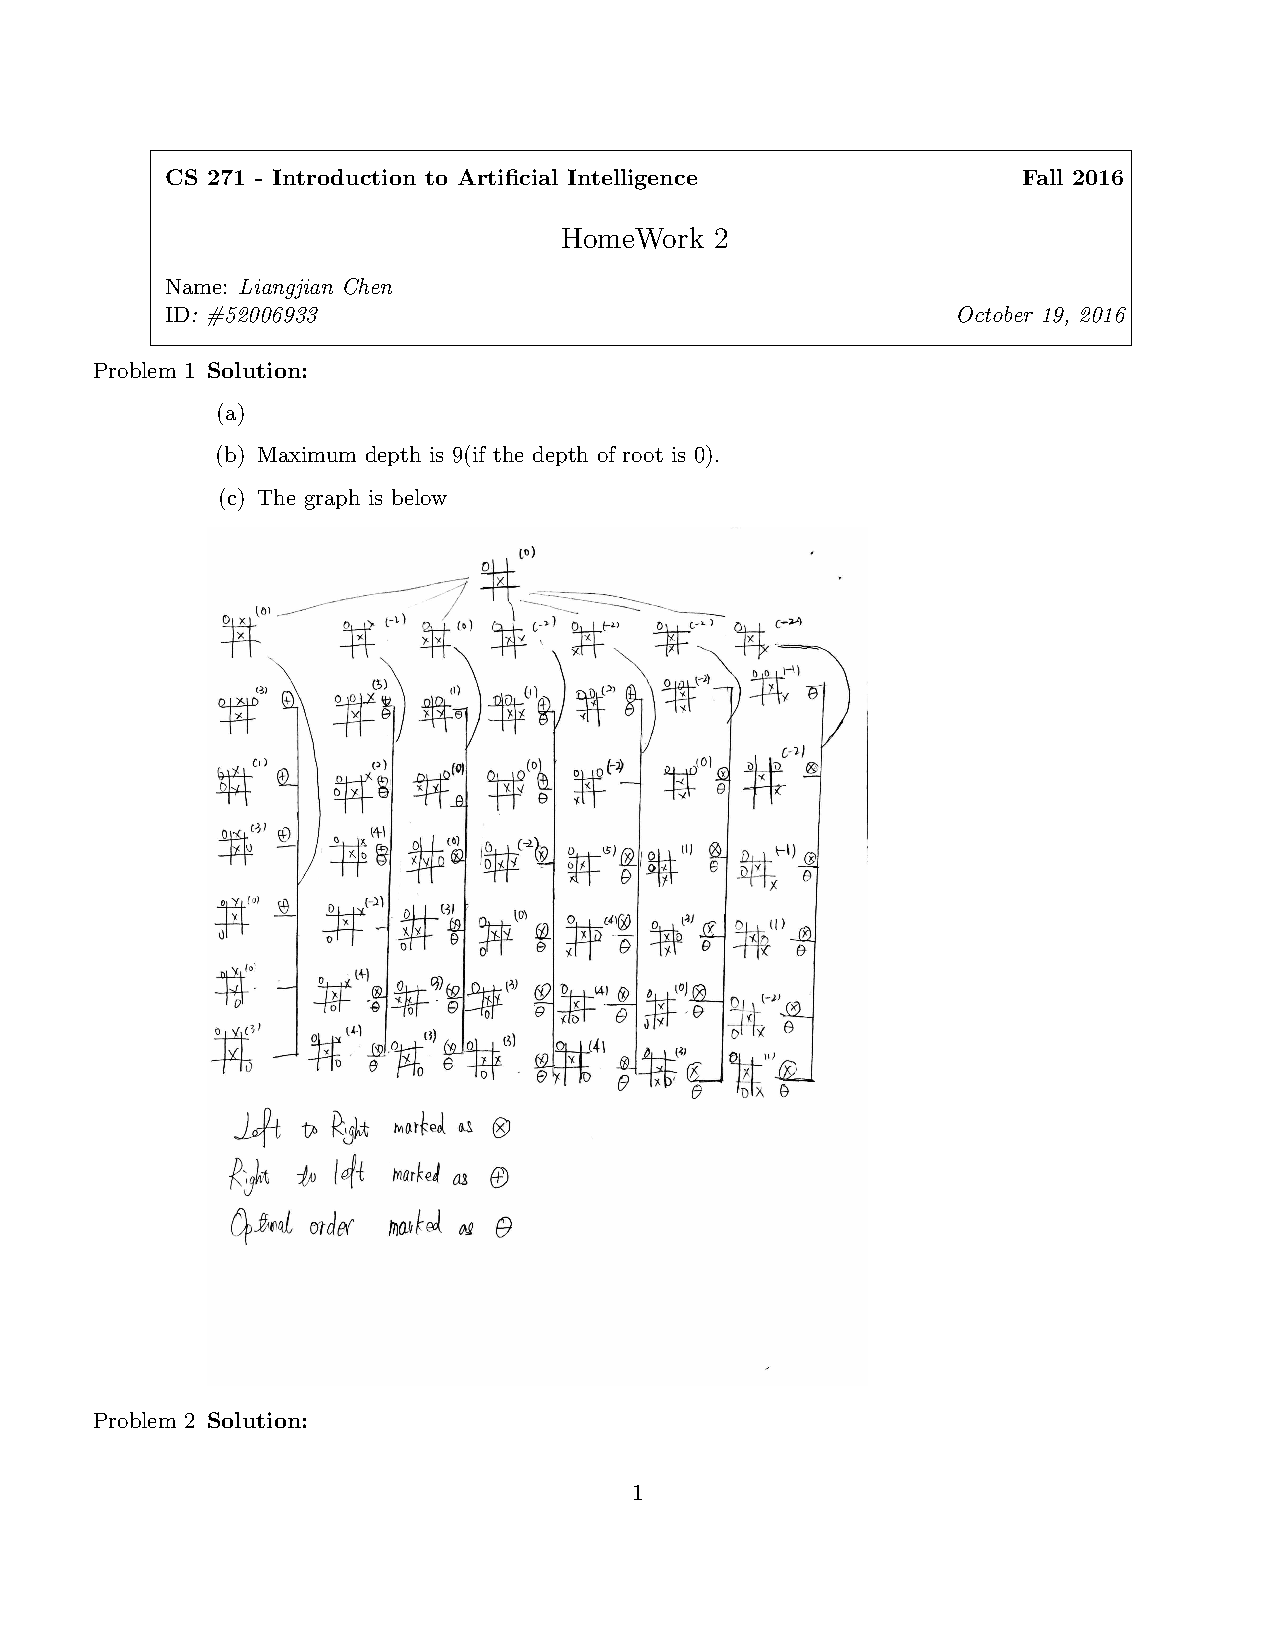
\includegraphics[width=2  in]{1.jpg}
		\item Yes
		\item No
	\end{enumerate}
\item[Problem 5]\textbf{Solution:}\par
	\begin{enumerate}
		\item New Domain as following:\\
		$D_2,D_3 = \{3,4,5,6,7,8,9\}$ \\
		$D_4,D_5,D_6,D_7 = \{5,6,7,8,9\}$ \\
		$D_8,D_9,...,D_{15} = \{7,8,9\}$
		\item One solution is following:\\
		$X_1 = 1$ \\
		$X_2,X_3 = 3$ \\
		$X_4,X_5,X_6,X_7 = 5$ \\
		$X_8,X_9,...,X_{15} = 7$
		\item from small to large
		\item assume $d$ is the size of domain, $O(15 * d^2) = O(d^2)$
	\end{enumerate}
\item[Problem 6]\textbf{Solution:}\par
	734 + 734 = 1468
\item[Problem 7]\textbf{Solution:}\par
	\begin{enumerate}
		\item variable elimination
		\item variable elimination
		\item variable elimination
	\end{enumerate}


\end{enumerate}
\end{document}
